\documentclass[12pt]{article}
\usepackage{geometry}
\geometry{a4paper, margin=1in}
\usepackage{graphicx}
\usepackage{booktabs}
\usepackage{hyperref}
\hypersetup{colorlinks=true, linkcolor=blue, urlcolor=blue}
\usepackage{natbib}
\bibliographystyle{apa}
\usepackage{times}

\begin{document}

\title{Workplace Design for TechSoft Inc.: A Post-Pandemic Strategy}
\author{}
\date{}
\maketitle

\begin{abstract}
This report outlines a comprehensive plan for designing a post-pandemic office workspace for TechSoft Inc., a hypothetical software development company. It addresses the organization's vision, mission, and operational framework, reviews 2025 workplace trends and best practices, analyzes current space planning, and provides evidence-based recommendations to enhance productivity and business success. The report leverages AI tools for efficiency, Python for data visualization, and LaTeX for professional presentation, ensuring a cost-effective approach.
\end{abstract}

\section{Introduction to the Case Study}
TechSoft Inc. is a hypothetical software development company based in San Francisco, California, designed to reflect the needs of a modern, post-pandemic workplace.

\subsection{Vision and Mission}
\textbf{Vision}: To be a global leader in software innovation, empowering businesses with cutting-edge technology while fostering employee well-being and flexibility.\\
\textbf{Mission}: To deliver high-quality, customized software solutions that drive business growth, through a commitment to excellence, collaboration, and continuous improvement.

\subsection{Organizational Structure}
TechSoft Inc. employs a flat hierarchy with cross-functional teams organized around projects. Each team includes developers, designers, testers, and a project manager, supported by HR, finance, and marketing functions.

\subsection{Business Nature and Target Customers}
The company specializes in developing web and mobile applications, enterprise software, and cloud solutions. Its target customers include small to medium-sized enterprises (SMEs), startups, and large corporations in industries such as finance, healthcare, retail, and education.

\subsection{Facilities and Systems}
The office features flexible workstations, meeting rooms with video conferencing, breakout areas, a cafeteria, and recreational spaces. Systems include cloud-based tools like Jira for project management, Slack for communication, and GitHub for version control.

\subsection{Business Processes}
TechSoft Inc. follows an agile methodology with sprints, daily stand-ups (virtual or in-person), sprint planning, and retrospectives. Client engagement involves consultation, requirement gathering, prototyping, development, testing, deployment, and maintenance.

\section{Literature Review}
This section synthesizes current research on workplace design, focusing on trends, best practices, and their impact on productivity and business success.

\subsection{Business Trends for 2025}
Research suggests that 2025 workplace trends emphasize hybrid work models, employee well-being, technology integration, and sustainability. According to \citet{gensler2025}, immersive experiences that engage all senses are replacing one-dimensional designs, promoting emotional connections and Hawkins{}. \citet{hbr2025} highlights the need for a future-ready workforce and AI adoption, with 56\% of office meetings being hybrid \citep{gensler2024}. Sustainability is also a priority, with eco-friendly materials and energy-efficient designs gaining traction \citep{edge2025}.

\subsection{Best Practices in Workplace Planning}
Post-pandemic workplace planning focuses on flexibility, health, and technology. \citet{gallup2025} emphasizes clear communication and change management, while \citet{gensler2023} advocates for indoor-outdoor synergy and spaces for reflection. Best practices include:
\begin{itemize}
    \item Flexible layouts with hot-desking and bookable spaces.
    \item Advanced HVAC systems and touchless technology for safety.
    \item Biophilic design with natural light and plants.
    \item Technology for seamless hybrid collaboration.
\end{itemize}

\subsection{Workplace Planning and Staff Productivity}
Studies show that workplace design significantly impacts productivity. \citet{sketchstudios2023} reports that poorly designed offices cost UK businesses up to £135 billion annually, with employees 19\% more productive in better environments. Natural light, ergonomic furniture, and quiet spaces enhance focus and reduce stress \citep{haiken2023}. However, \citet{ciphr2023} notes that 37\% of workers in open-plan offices report decreased productivity due to noise.

\subsection{Workplace Planning and Business Success}
Effective workplace design drives business success by attracting talent, boosting productivity, and enhancing client perceptions. \citet{moneypenny2025} states that well-designed spaces improve talent acquisition and retention. \citet{officespace2019} found that 85\% of employees believe clients judge companies based on workplace design, and 79\% are more likely to join a company with a well-designed office.

\section{Analysis of Current Space Planning}
TechSoft Inc.'s hypothetical pre-pandemic office features an open-plan layout with rows of desks, private manager offices, meeting rooms, a break room, and a recreational area with a ping-pong table. This design has several shortcomings:
\begin{itemize}
    \item \textbf{Open-Plan Limitations}: Lacks support for social distancing and privacy, increasing distractions \citep{ciphr2023}.
    \item \textbf{Inflexibility}: Fixed desks do not accommodate hybrid work schedules.
    \item \textbf{Technology Gaps}: Insufficient video conferencing tools for hybrid meetings.
    \item \textbf{Limited Wellness Features}: Few spaces for relaxation or access to nature.
\end{itemize}

\begin{figure}[h]
    \centering
    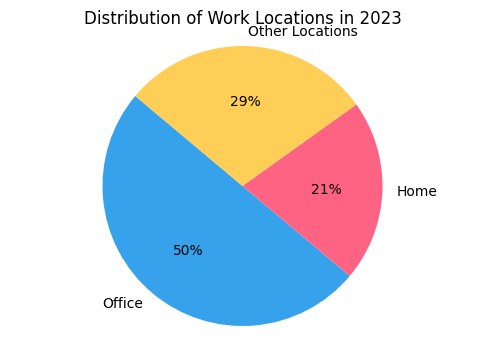
\includegraphics[width=0.5\textwidth]{work_locations.png}
    \caption{Distribution of Work Locations in 2023 \citep{gensler2024}}
\end{figure}

\section{Explanation of Findings}
The current office design is inadequate for post-pandemic needs. Open-plan layouts hinder focused work and pose health risks due to close proximity. The lack of flexible workstations limits adaptability for hybrid schedules, where employees spend 50\% of their time in the office and 21\% at home \citep{gensler2024}. Inadequate technology fails to support the 56\% of meetings that are hybrid, reducing collaboration efficiency. The absence of wellness-focused spaces neglects employee mental health, which is critical for productivity \citep{forbes2019}.

\section{Recommendations}
To address these issues, TechSoft Inc. should adopt a hybrid-friendly, wellness-centric office design:
\begin{itemize}
    \item \textbf{Flexible Workspaces}: Implement hot-desking and bookable spaces using mobile apps for scheduling \citep{yourworkspace2025}.
    \item \textbf{Technology Integration}: Equip meeting rooms with advanced video conferencing tools to support hybrid meetings.
    \item \textbf{Private Areas}: Create pods or booths for focused work, addressing the 35\% of time spent working alone \citep{gensler2024}.
    \item \textbf{Biophilic Design}: Incorporate plants, natural light, and outdoor access to enhance well-being \citep{haiken2023}.
    \item \textbf{Health and Safety}: Install advanced HVAC systems and touchless technology \citep{workdesign2021}.
    \item \textbf{Modular Furniture}: Use adaptable, easy-to-sanitize furniture \citep{vicus2024}.
\end{itemize}
These changes will improve productivity by reducing distractions and stress, and enhance business success by attracting talent and creating a positive client impression \citep{moneypenny2025}.

\section{Conclusion}
The proposed workplace design for TechSoft Inc. aligns with 2025 trends and best practices, addressing the limitations of the current layout. By prioritizing flexibility, technology, and well-being, the new design will enhance staff productivity and contribute to business success.

\begin{table}[h]
    \centering
    \caption{Key Workplace Design Trends for 2025}
    \begin{tabular}{p{5cm}p{10cm}}
        \toprule
        \textbf{Trend} & \textbf{Description} \\
        \midrule
        Hybrid Work Models & Flexible spaces for in-office and remote work \citep{gensler2025}. \\
        Employee Well-Being & Biophilic design and wellness rooms to reduce stress \citep{haiken2023}. \\
        Technology Integration & Advanced tools for hybrid collaboration \citep{gensler2024}. \\
        Sustainability & Eco-friendly materials and energy-efficient designs \citep{edge2025}. \\
        \bottomrule
    \end{tabular}
\end{table}

\bibliography{references}
\end{document}